In this section, we analyze the performance of \pred, \predt, \dptg, \ad, \ts, and \linucb\ when the weak demonstrator $\pi^w$ is \ts, \linucb, or \unif. We again consider the linear bandit setting discussed in \Cref{sec:short-horizon}. 
% Recall that the linear bandit setting consist of horizon $n=25$, $\Mpr = 200000$, $\Mts = 200$, $A=10$, and $d=2$. Finally, 
We show the cumulative regret by the above baselines in \Cref{fig:TS-collection}, \ref{fig:linucb-collection}, and \ref{fig:linucb-collection} when data is collected through \ts, \linucb, and \unif\ respectively. We first state the main finding below:
%
% \textbf{Outcomes:} We discuss the main outcomes of our experimental results for different data collection:
%
\begin{tcolorbox}
    \customfinding The \pred\ (\gt) excels in exploiting the underlying latent structure and reward correlation from in-context data when the data diversity is high.
\end{tcolorbox}
%
% \noindent
% \textbf{(1)} The \pred\ (\gt) excels in exploiting the underlying latent structure and reward correlation when the data diversity is high.
%
% \textbf{(2)} The \pred\ (\gt) fails to exploit the underlying latent structure and reward correlation when the data diversity is less.
%
% \textbf{(3)} The \pred\ (\gt) has lower regret compared to \dptg\ in all settings. \ad\ outperforms \pred\ (\gt) when data is collected by \linucb.
%
% \begin{figure}[!hbt]
% \centering
% \begin{tabular}{ccc}
% \subfigure[\ts\ data collection ]{\hspace*{-1.5em}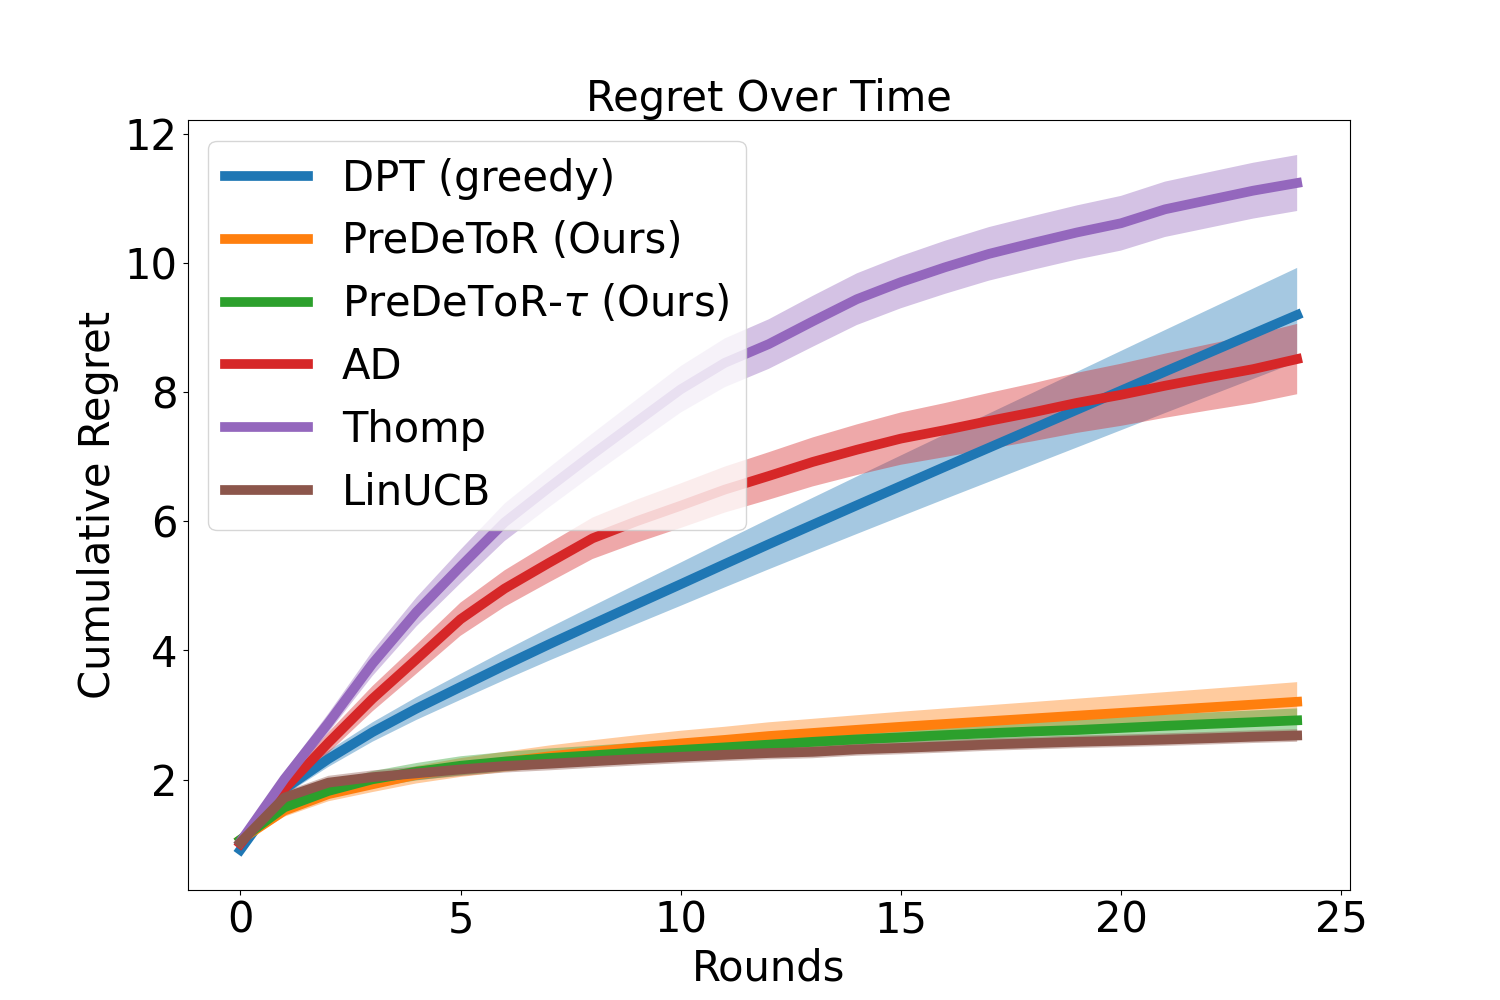
\includegraphics[scale = 0.13]{img/Neurips/weak_Dem/linTS_lr0.00015_do0_embd32_layer4_head4_envs100000_hists1_samples1_var0.3_cov0.0_H25_d10_lind2_seed1_testcov0.0_hor25.pkl.png}\label{fig:TS-collection}} &
% %%%%%%%%%%
% \hspace*{-1.5em}\subfigure[\linucb\ data collection]{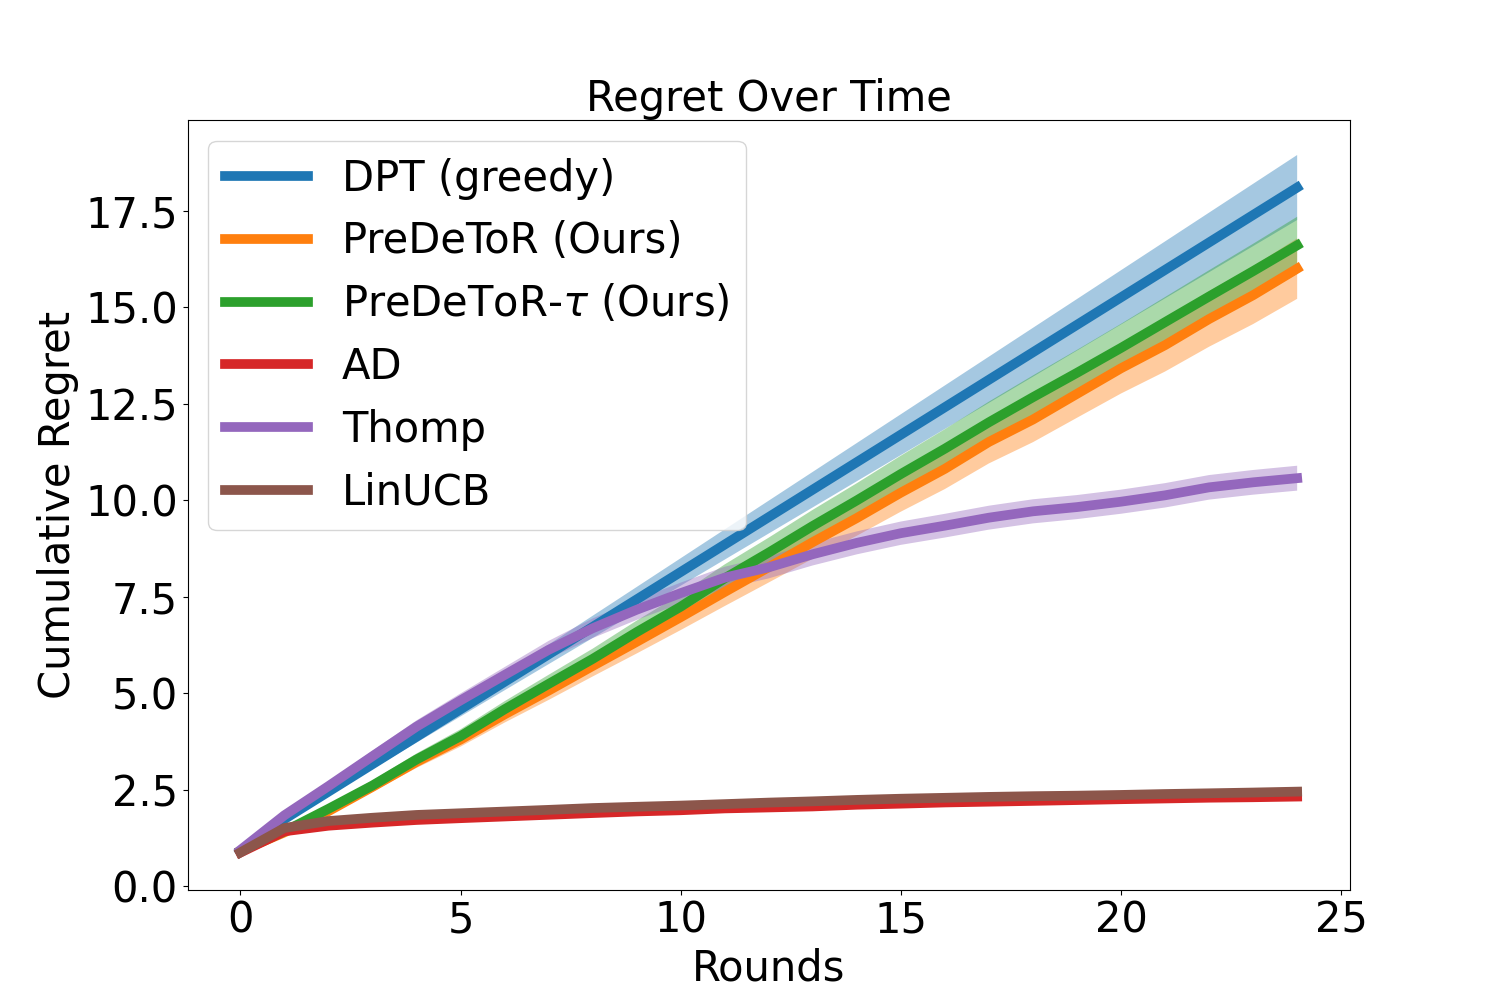
\includegraphics[scale = 0.13]{img/Neurips/weak_Dem/linucb_lr0.00015_do0_embd32_layer4_head4_envs100007_hists1_samples1_var0.3_cov0.0_H25_d10_lind2_seed1_testcov0.0_hor25.pkl.png} \label{fig:linucb-collection}} &
% %%%%%%%%%%%%%%%%%%%%%%%
% \subfigure[\unif\ data collection]{\hspace*{-1.5em}\includegraphics[scale = 0.13]{img/Neurips/weak_Dem/linUnif_lr0.00015_do0_embd32_layer4_head4_envs100009_hists1_samples1_var0.3_cov0.0_H25_d10_lind2_seed1_testcov0.0_hor25.pkl.png}\label{fig:unif-collection}} 
% \end{tabular}
% \caption{Data Collection with various algorithms and Performance analysis}
% \label{fig:data-collection}
% \end{figure}
%
% \vspace*{-1em}
\begin{figure}[!hbt]
\centering
\begin{subfigure}[b]{0.32\textwidth}
   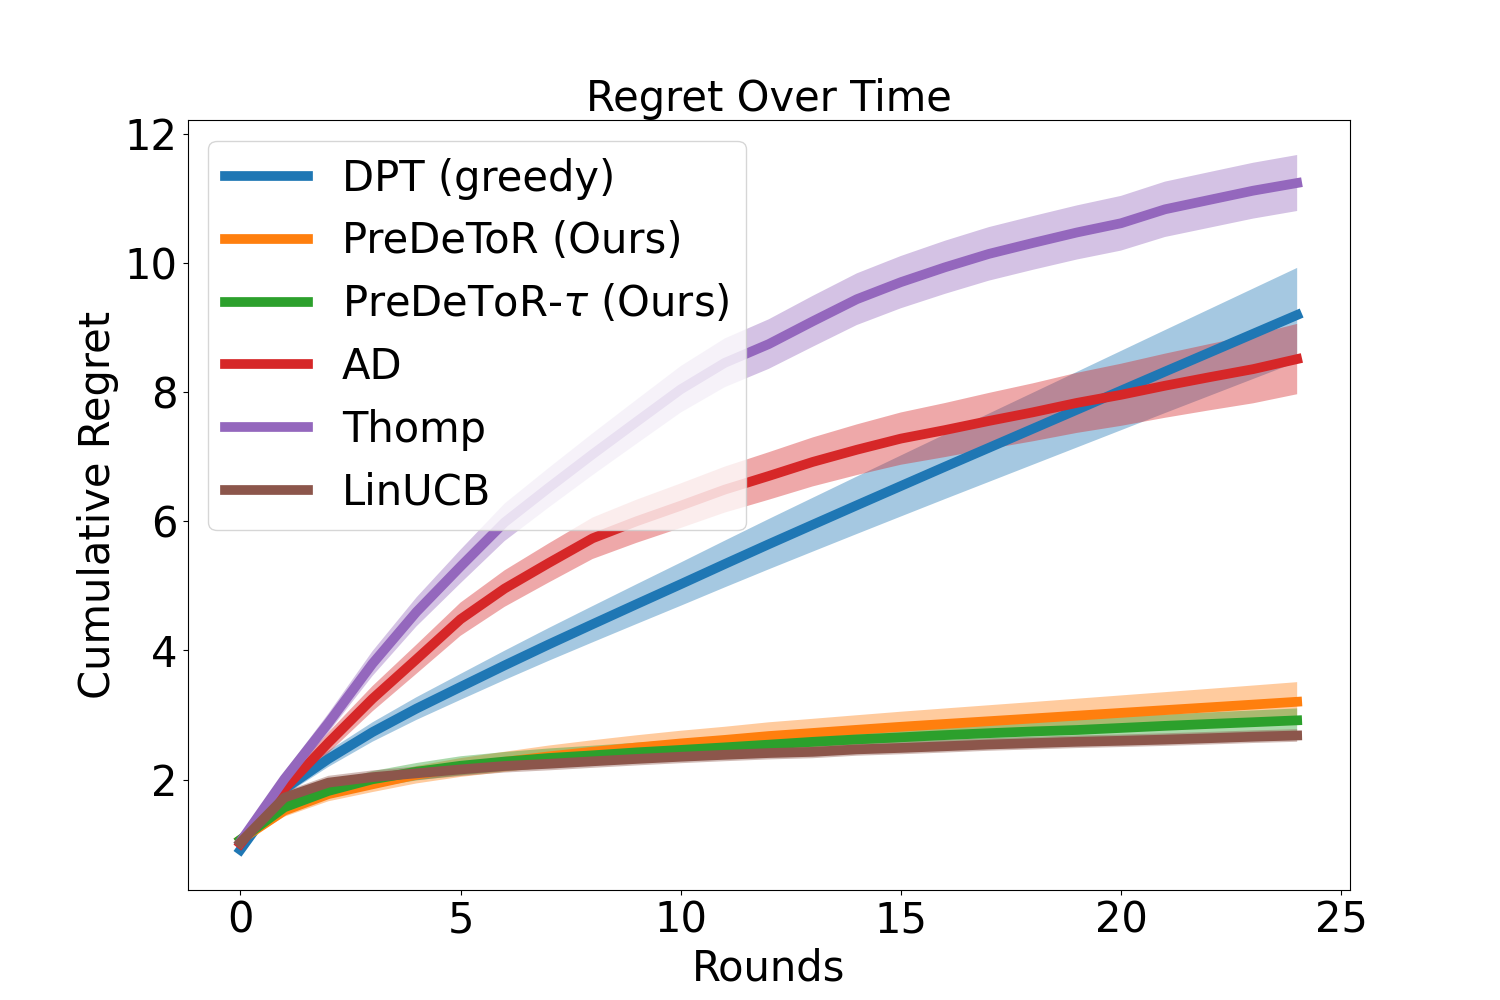
\includegraphics[scale=0.1]{img/Neurips/weak_Dem/linTS_lr0.00015_do0_embd32_layer4_head4_envs100000_hists1_samples1_var0.3_cov0.0_H25_d10_lind2_seed1_testcov0.0_hor25.pkl.png}
   \caption{\ts\ data collection}
   \label{fig:TS-collection}
\end{subfigure}%
\begin{subfigure}[b]{0.32\textwidth}
   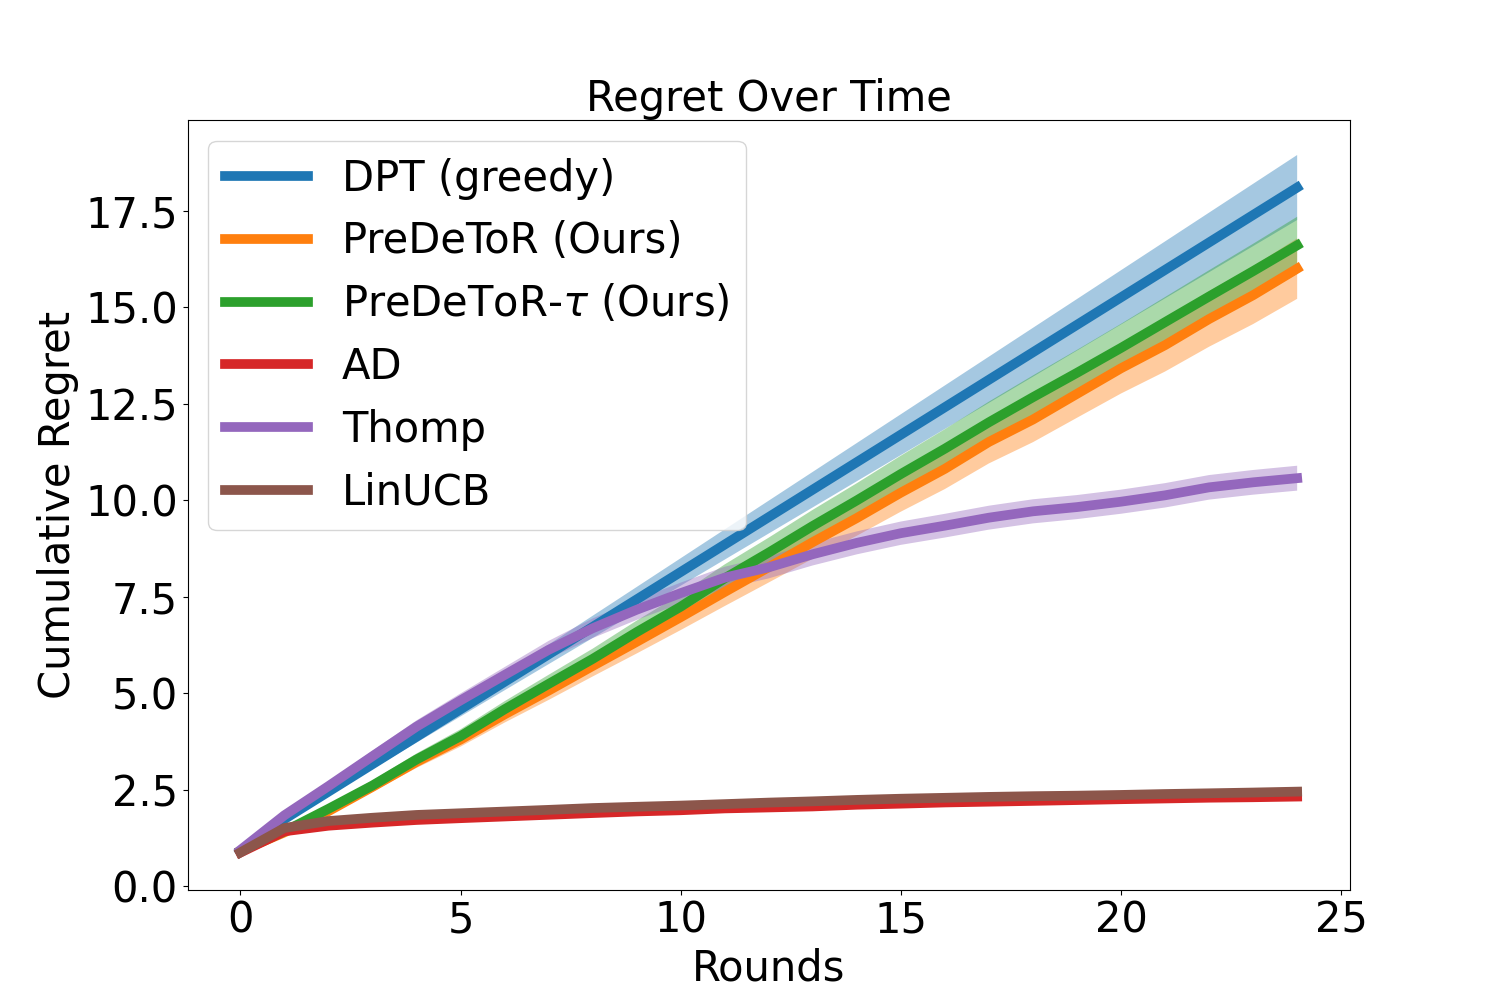
\includegraphics[scale=0.1]{img/Neurips/weak_Dem/linucb_lr0.00015_do0_embd32_layer4_head4_envs100007_hists1_samples1_var0.3_cov0.0_H25_d10_lind2_seed1_testcov0.0_hor25.pkl.png}
   \caption{\linucb\ data collection}
   \label{fig:linucb-collection}
\end{subfigure}%
\begin{subfigure}[b]{0.32\textwidth}
   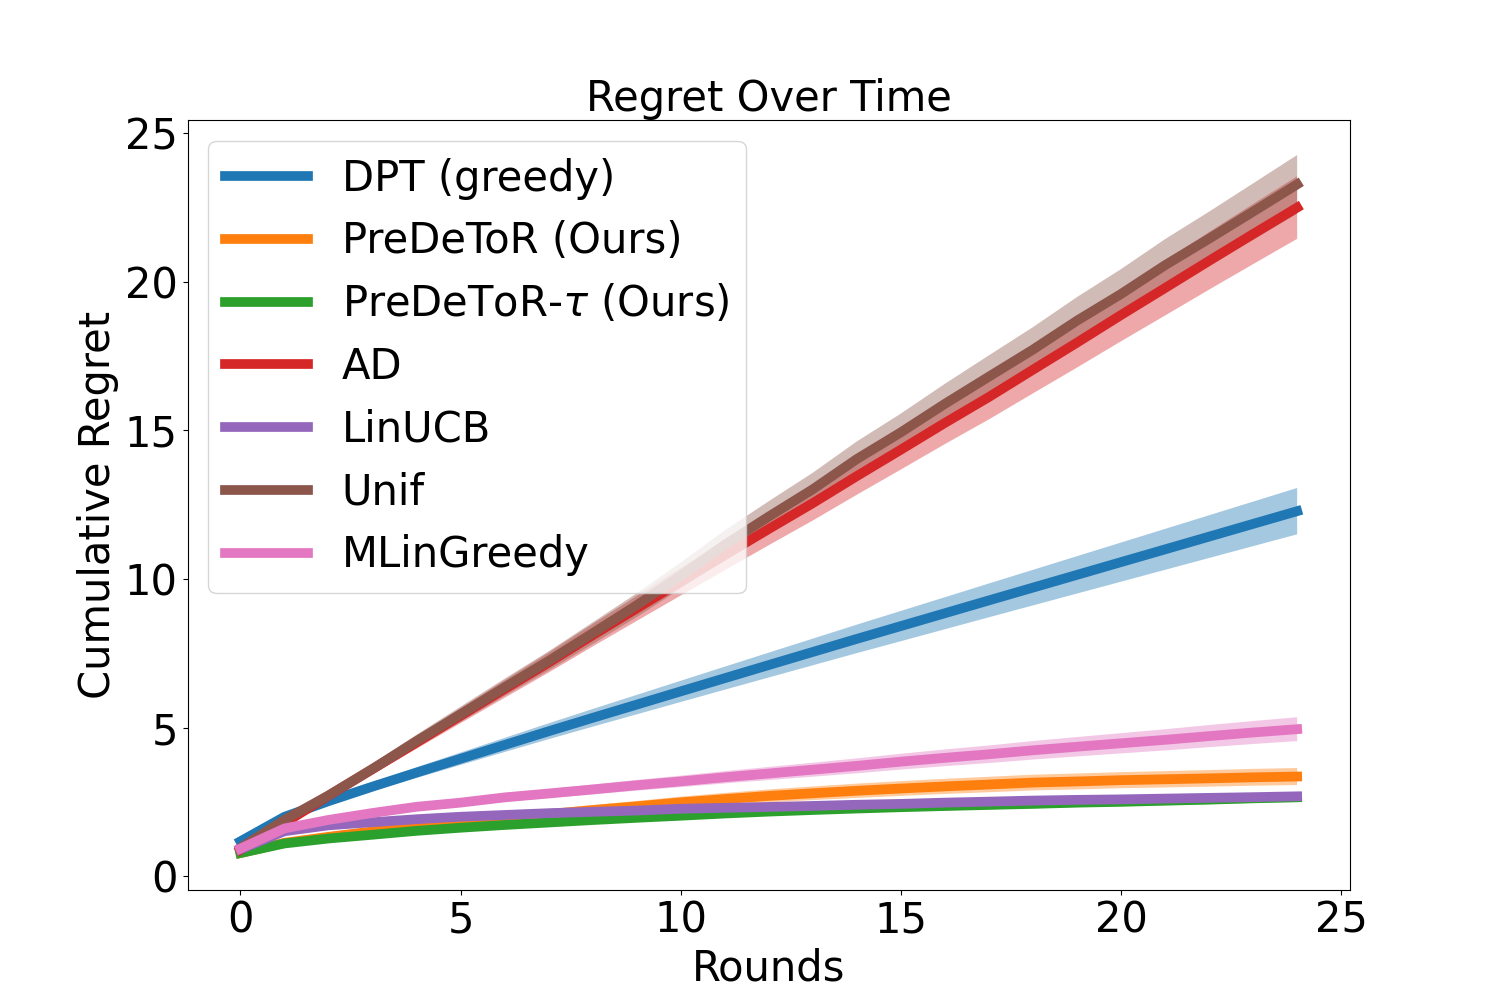
\includegraphics[scale=0.1]{img/Neurips/weak_Dem/linunif_lr0.00015_do0_embd32_layer4_head4_envs100009_hists1_samples1_var0.3_cov0.0_H25_d10_lind2_seed1_testcov0.0_hor25.pkl.png}
   \caption{\unif\ data collection}
   \label{fig:unif-collection}
\end{subfigure}
% \vspace*{-1em}
\caption{Data Collection with various algorithms and Performance analysis}
\label{fig:data-collection}
\end{figure}
% \vspace*{-2em}

\textbf{Experimental Result:} We observe these outcomes in \Cref{fig:data-collection}. In \Cref{fig:TS-collection} we see that the $A$-actioned \ts\ is explorative enough as it does not explore with the knowledge of feature representation. 
%
So it pulls the sub-optimal actions sufficiently high number of times before discarding them in favor of the optimal action.
%
Therefore the training data is diverse enough so that \pred\ (\gt) can predict the reward vectors for actions sufficiently well. Consequently, \pred\ (\gt) almost matches the \linucb\ algorithm. Both \dptg\ and \ad perform poorly in this setting.
%
%

In \Cref{fig:linucb-collection} we see that the \linucb\ algorithm is not explorative enough as it explores with the knowledge of feature representation and quickly discards the sub-optimal actions in favor of the optimal action. Therefore the training data is not diverse enough so that \pred\ (\gt) is not able to correctly predict the reward vectors for actions. Note that \dptg\ also performs poorly in this setting when it is not provided with the optimal action information during training. The \ad\ matches the performance of its demonstrator \linucb\ because of its training procedure of predicting the next action of the demonstrator. 
%

Finally, in \Cref{fig:unif-collection} we see that the $A$-armed \unif\ is fully explorative as it does not intend to minimize regret (as opposed to \ts) and does not explore with the knowledge of feature representation. Therefore the training data is very diverse which results in \pred\ (\gt) being able to predict the reward vectors for actions very well. Consequently, \pred\ (\gt) perfectly matches the \linucb\ algorithm. Note that \ad\ performs the worst as it matches the performance of its demonstrator whereas the performance of \dptg\ suffers due to the lack of information on the optimal action during training.

We also empirically study the test performance of \pred\ (\gt) in $K$-armed bandit setting when there is no structure across arms in \Cref{sec:k_arms_dpt}, against the original \dpt\ in \Cref{sec:k_arms_dpt}, 
%
in other \textit{non-linear} bandit settings such as bilinear bandits (\Cref{sec:bilinear}), latent bandits (\Cref{sec:latent}), draw a connection between \pred\ and Bayesian estimators (\Cref{sec:und}), and perform sensitivity and ablation studies in \Cref{sec:lim}, \ref{sec:dimension}, \ref{sec:heads}, \ref{sec:envs}. 
%
% We discuss data collection algorithms in \Cref{sec:data-collection} and the offline setting in \Cref{sec:offline}.
Due to space constraints, we refer the interested reader to the relevant section in the appendices.